\documentclass[tikz,border=5pt]{standalone}
\usepackage{amsmath,amssymb}
\usetikzlibrary{arrows.meta,positioning,calc}
\begin{document}
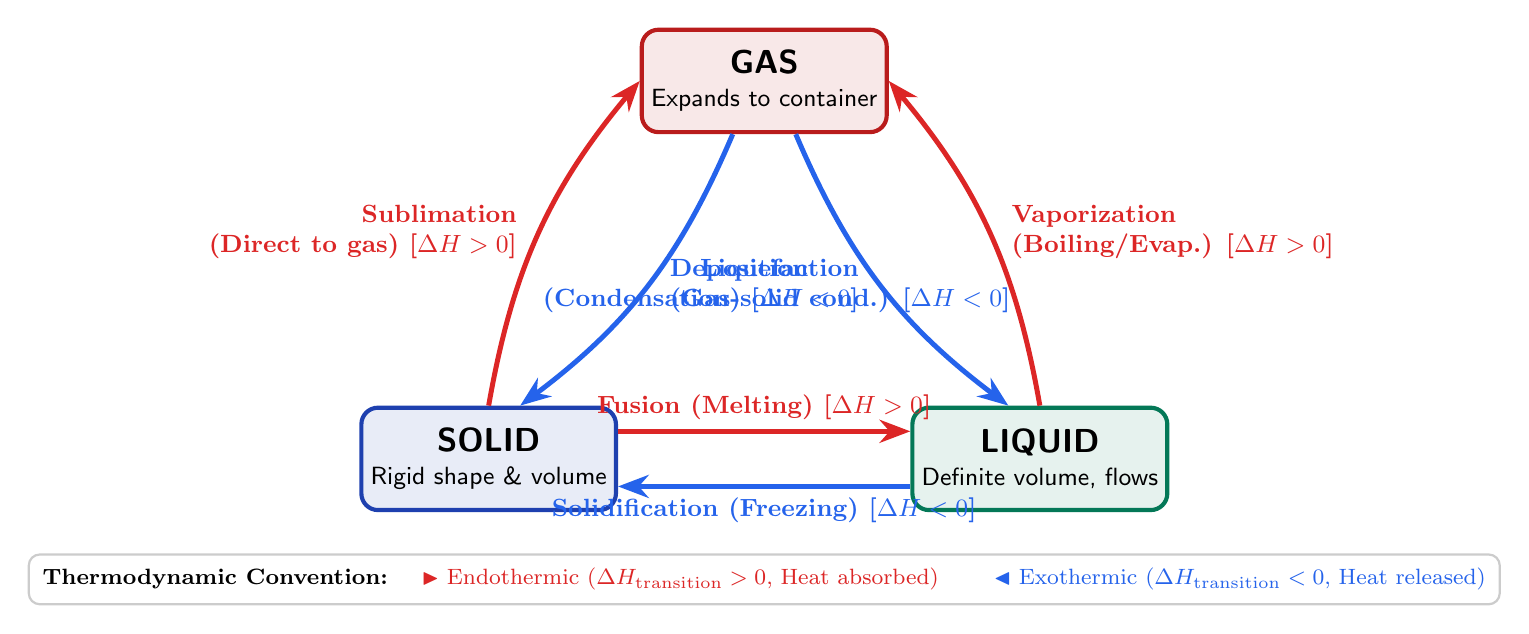
\begin{tikzpicture}[>=Stealth, font=\sffamily, thick]
  \definecolor{solcolor}{HTML}{1E40AF}
  \definecolor{liqcolor}{HTML}{047857}
  \definecolor{gascolor}{HTML}{B91C1C}
  \definecolor{arrowheat}{HTML}{DC2626}
  \definecolor{arrowcool}{HTML}{2563EB}

  \node[draw=solcolor, fill=solcolor!10, rounded corners=6pt, minimum width=2.8cm, minimum height=1.3cm, align=center, line width=1.5pt] (sol) at (0,0) {\textbf{\large SOLID}\\\small Rigid shape \& volume};
  \node[draw=liqcolor, fill=liqcolor!10, rounded corners=6pt, minimum width=2.8cm, minimum height=1.3cm, align=center, line width=1.5pt] (liq) at (7,0) {\textbf{\large LIQUID}\\\small Definite volume, flows};
  \node[draw=gascolor, fill=gascolor!10, rounded corners=6pt, minimum width=2.8cm, minimum height=1.3cm, align=center, line width=1.5pt] (gas) at (3.5,4.8) {\textbf{\large GAS}\\\small Expands to container};

  % Solid <-> Liquid
  \draw[->, arrowheat, line width=1.8pt] ([yshift=3.5mm]sol.east) -- node[above, text=arrowheat, font=\bfseries\small] {Fusion (Melting) [$\Delta H > 0$]} ([yshift=3.5mm]liq.west);
  \draw[<-, arrowcool, line width=1.8pt] ([yshift=-3.5mm]sol.east) -- node[below, text=arrowcool, font=\bfseries\small] {Solidification (Freezing) [$\Delta H < 0$]} ([yshift=-3.5mm]liq.west);

  % Liquid <-> Gas
  \draw[->, arrowheat, line width=1.8pt] (liq.north) to[bend right=15] node[right=4pt, text=arrowheat, font=\bfseries\small, align=left] {Vaporization\\(Boiling/Evap.) [$\Delta H > 0$]} (gas.east);
  \draw[<-, arrowcool, line width=1.8pt] ([xshift=-4mm]liq.north) to[bend left=15] node[left=4pt, text=arrowcool, font=\bfseries\small, align=right] {Liquefaction\\(Condensation) [$\Delta H < 0$]} ([xshift=4mm]gas.south);

  % Solid <-> Gas
  \draw[->, arrowheat, line width=1.8pt] (sol.north) to[bend left=15] node[left=4pt, text=arrowheat, font=\bfseries\small, align=right] {Sublimation\\(Direct to gas) [$\Delta H > 0$]} (gas.west);
  \draw[<-, arrowcool, line width=1.8pt] ([xshift=4mm]sol.north) to[bend right=15] node[right=4pt, text=arrowcool, font=\bfseries\small, align=left] {Deposition\\(Gas-solid cond.) [$\Delta H < 0$]} ([xshift=-4mm]gas.south);

  % Legend
  \node[anchor=north, draw=gray!40, fill=white, rounded corners=4pt, inner sep=5pt, font=\footnotesize] at (3.5, -1.2) {
    \textbf{Thermodynamic Convention:} \quad
    {\color{arrowheat}$\blacktriangleright$ Endothermic ($\Delta H_{\text{transition}} > 0$, Heat absorbed)} \qquad
    {\color{arrowcool}$\blacktriangleleft$ Exothermic ($\Delta H_{\text{transition}} < 0$, Heat released)}
  };
\end{tikzpicture}
\end{document}
